\noindent Ως τελευταίο μέρος της εργασίας και περισσότερο για λόγους πειραματισμού, αποφασίσαμε να τρέξουμε τον κώδικα μας στην πλατφόρμα Google Cloud Platform αξιοποιώντας την πρόσβαση που μας παρέχει σε πιο σύγχρονο εξοπλισμό. Παρακάτω παρατίθενται τα τεχνικά χαρακτηριστικά του virtual machine που δημιουργήσαμε:

\begin{verbatim}
======== CPU ========
Architecture:          x86_64
CPU op-mode(s):        32-bit, 64-bit
Byte Order:            Little Endian
CPU(s):                4
On-line CPU(s) list:   0-3
Thread(s) per core:    2
Core(s) per socket:    2
Socket(s):             1
NUMA node(s):          1
Vendor ID:             GenuineIntel
CPU family:            6
Model:                 45
Model name:            Intel(R) Xeon(R) CPU @ 2.60GHz
Stepping:              7
CPU MHz:               2600.000
BogoMIPS:              5200.00
Hypervisor vendor:     KVM
Virtualization type:   full
L1d cache:             32K
L1i cache:             32K
L2 cache:              256K
L3 cache:              20480K

======== RAM ========
MemTotal:       16425608 kB

======== GPU ========
Device 0: "Tesla V100-SXM2-16GB"
  CUDA Driver Version / Runtime Version          10.0 / 10.0
  CUDA Capability Major/Minor version number:    7.0
  Total amount of global memory:                 16130 MBytes (16914055168 bytes)
  (80) Multiprocessors, ( 64) CUDA Cores/MP:     5120 CUDA Cores
  GPU Max Clock rate:                            1530 MHz (1.53 GHz)
  Memory Clock rate:                             877 Mhz
  Memory Bus Width:                              4096-bit
  L2 Cache Size:                                 6291456 bytes
  Maximum Texture Dimension Size (x,y,z)         1D=(131072), 2D=(131072, 65536), 
                                                 3D=(16384, 16384, 16384)
  Maximum Layered 1D Texture Size, (num) layers  1D=(32768), 2048 layers
  Maximum Layered 2D Texture Size, (num) layers  2D=(32768, 32768), 2048 layers
  Total amount of constant memory:               65536 bytes
  Total amount of shared memory per block:       49152 bytes
  Total number of registers available per block: 65536
  Warp size:                                     32
  Maximum number of threads per multiprocessor:  2048
  Maximum number of threads per block:           1024
  Max dimension size of a thread block (x,y,z): (1024, 1024, 64)
  Max dimension size of a grid size    (x,y,z): (2147483647, 65535, 65535)
  Maximum memory pitch:                          2147483647 bytes
  Texture alignment:                             512 bytes
  Concurrent copy and kernel execution:          Yes with 2 copy engine(s)
  Run time limit on kernels:                     No
  Integrated GPU sharing Host Memory:            No
  Support host page-locked memory mapping:       Yes
  Alignment requirement for Surfaces:            Yes
  Device has ECC support:                        Enabled
  Device supports Unified Addressing (UVA):      Yes
  Device supports Compute Preemption:            Yes
  Supports Cooperative Kernel Launch:            Yes
  Supports MultiDevice Co-op Kernel Launch:      Yes
  Device PCI Domain ID / Bus ID / location ID:   0 / 0 / 4
\end{verbatim}

\subsection*{Αποτελέσματα}

\noindent Παρακάτω παρατίθενται οι μετρήσεις που προέκυψαν από την εκτέλεση του κώδικα των δύο τελευταίων ερωτημάτων στο νέο περιβάλλον. Σε αυτό το σημείο πρέπει να αναφερθεί ότι δεν προχωρήσαμε σε βελτιστοποίηση του προγράμματος ώστε να ανταποκρίνεται καλύτερα στις πιθανές απαιτήσεις που θέτει η εκτέλεσή του σε μία αρκετά μεταγενέστερη κάρτα γραφικών, παραμόνο τρέξαμε τον ίδιο κώδικα για να δούμε πως θα συμπεριφερθεί στο νέο υλικό.

\begin{center}
    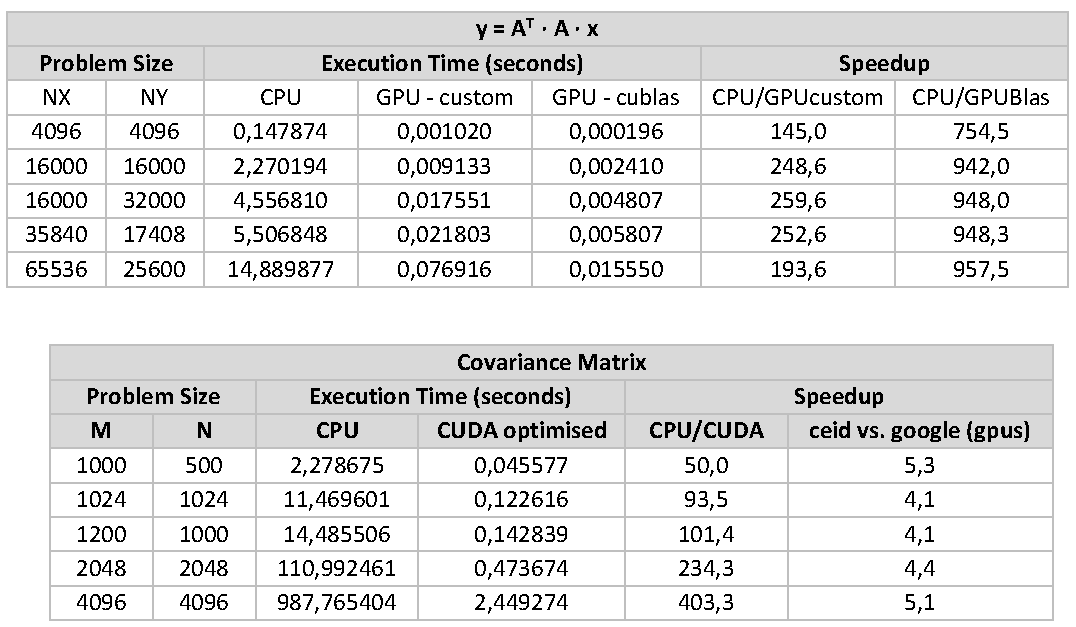
\includegraphics[scale=0.9]{./figures/3_covar/google}
\end{center}

\noindent Με μία πρώτη ματιά παρατηρούμε ότι και μόνο η μετάβαση σε μία πιο ισχυρή κάρτα γραφικών είναι ικανή να μας δώσει πολλαπλάσιο speedup από αυτό που πετυχαίναμε. Επίσης είναι φανερό ότι η κυριότερη διαφορά έγκειται στην επεξεργαστική ισχύ της GPU και όχι της CPU αφού σε πολλές περιπτώσεις ο αρχικός επεξεργαστής κατέληγε σε μικρότερους χρόνους εκτέλεσης. Τέλος, πολλά από τα αρχικά συμπεράσματα ισχύουν και σε αυτήν την περίπτωση καθώς και εδώ βλέπουμε την υπεροχή της cuBLAS σε σχέση με την δική μας υλοποίηση ενώ παρατηρούμε ότι σε γενικές γραμμές, όσο μεγαλύτερο είναι το μέγεθος του προβλήματος τόσο καλύτερο speedup παίρνουμε. 